\documentclass[tikz, border=10pt]{standalone}
\usepackage{tikz}
\usepackage{xcolor}
\usepackage{amsmath}
\usetikzlibrary{arrows.meta, positioning, calc, shapes.geometric, backgrounds}

%%% Neon Lab color palette
\definecolor{tnblue}{RGB}{70, 115, 210}       % muted blue — existing infrastructure
\definecolor{tnmagenta}{RGB}{230, 0, 185}     % neon magenta — TinyNet nodes
\definecolor{tnlime}{RGB}{85, 240, 35}        % lime green — reroute arrows
\definecolor{tnorange}{RGB}{255, 148, 0}      % bright orange — warnings / vs badge
\definecolor{tnhotred}{RGB}{255, 50, 20}      % hot red — failures
\definecolor{tnpurple}{RGB}{165, 70, 255}     % neon purple — controller / metrics
\definecolor{tncyan}{RGB}{0, 225, 235}        % neon cyan — heartbeats
\definecolor{tngray}{RGB}{115, 120, 140}      % muted gray — existing edges / nodes
\definecolor{tnleftbg}{RGB}{20, 22, 34}       % dark blue-charcoal — left panel bg
\definecolor{tnrightbg}{RGB}{16, 26, 18}      % dark green-charcoal — right panel bg
\definecolor{tnmetricbg}{RGB}{10, 10, 16}     % near-black — metrics bar bg

\begin{document}
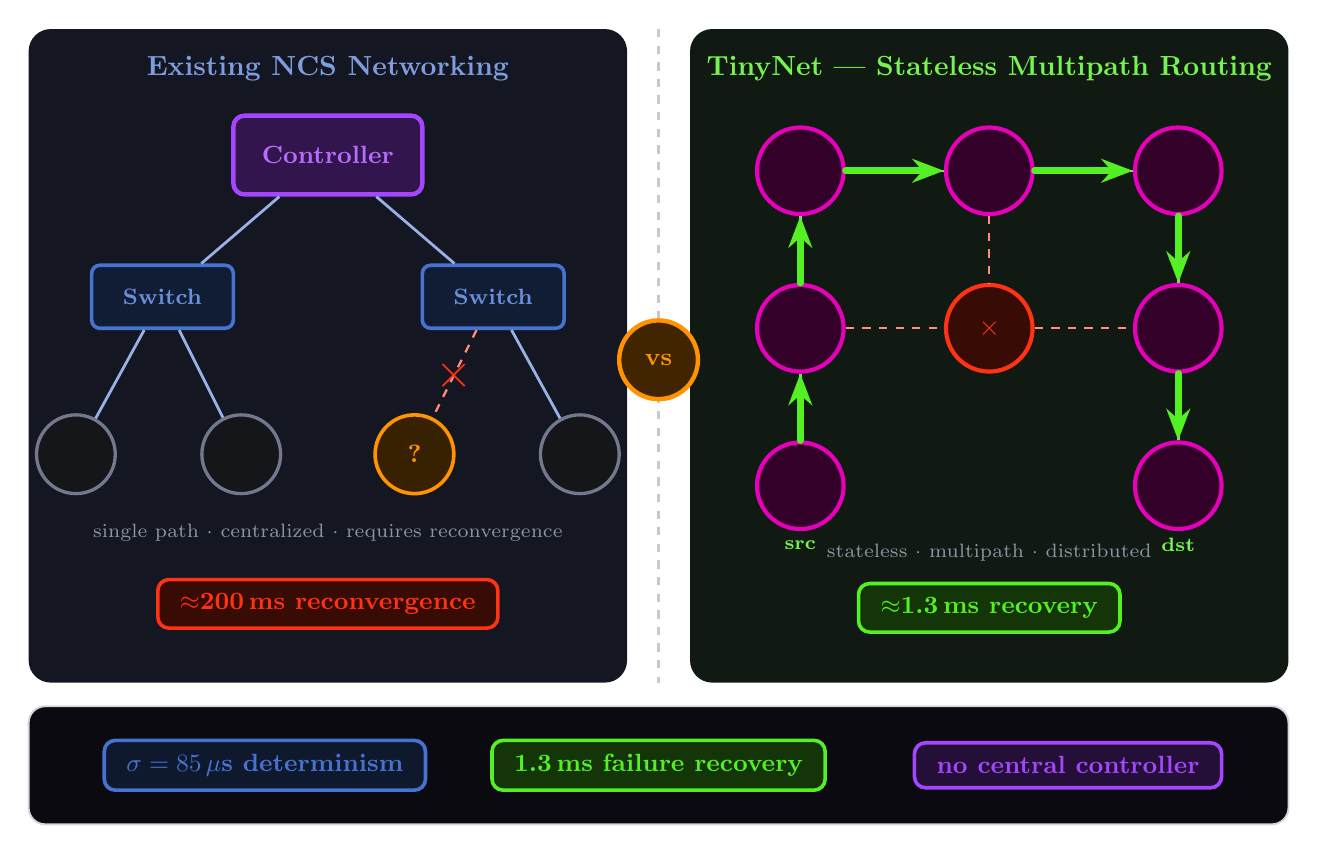
\begin{tikzpicture}[
  ctrlnode/.style={
    rectangle, rounded corners=4pt,
    draw=tnpurple, fill=tnpurple!30!black,
    minimum width=24mm, minimum height=10mm,
    line width=1.6pt,
    font=\small\bfseries, text=tnpurple!80!white
  },
  swnode/.style={
    rectangle, rounded corners=3pt,
    draw=tnblue, fill=tnblue!25!black,
    minimum width=18mm, minimum height=8mm,
    line width=1.3pt,
    font=\footnotesize\bfseries, text=tnblue!80!white
  },
  oldnode/.style={
    circle, draw=tngray, fill=tngray!18!black,
    minimum size=10mm, line width=1.2pt,
    font=\scriptsize\bfseries, text=tngray
  },
  alarmnode/.style={
    circle, draw=tnorange, fill=tnorange!22!black,
    minimum size=10mm, line width=1.3pt,
    font=\small\bfseries, text=tnorange
  },
  tnnode/.style={
    circle, draw=tnmagenta, fill=tnmagenta!22!black,
    minimum size=11mm, line width=1.5pt,
  },
  failnode/.style={
    circle, draw=tnhotred, fill=tnhotred!22!black,
    minimum size=11mm, line width=1.5pt,
    font=\normalsize\bfseries, text=tnhotred
  },
  treeedge/.style={draw=tnblue!55, line width=1.0pt},
  normaledge/.style={draw=tngray!55, line width=0.9pt},
  failedge/.style={draw=tnhotred!55, line width=0.8pt, dashed},
  reroutearrow/.style={
    draw=tnlime, line width=2.5pt,
    -{Stealth[length=4mm, width=3mm]},
    line cap=round, line join=round
  },
  waitarrow/.style={
    draw=tnorange, line width=1.5pt,
    -{Stealth[length=3mm]}, dashed
  },
  metricbox/.style={
    rectangle, rounded corners=4pt,
    draw=#1, fill=#1!22!black,
    line width=1.3pt,
    font=\small\bfseries, text=#1,
    inner xsep=8pt, inner ysep=5pt
  },
]

%% ================================================================
%% BACKGROUND PANELS
%% ================================================================
\fill[tnleftbg,  rounded corners=8pt]  (-0.3, -0.6) rectangle  (7.3, 7.7);
\fill[tnrightbg, rounded corners=8pt]   (8.1, -0.6) rectangle (15.7, 7.7);

%% ================================================================
%% LEFT PANEL: Existing NCS Networking
%% ================================================================

\node[font=\normalsize\bfseries, text=tnblue!70!white] at (3.5, 7.2)
  {Existing NCS Networking};

% Controller (top)
\node[ctrlnode] (ctrl) at (3.5, 6.1) {Controller};

% Switches (middle tier)
\node[swnode] (sw1) at (1.4, 4.3) {Switch};
\node[swnode] (sw2) at (5.6, 4.3) {Switch};

% Endpoint nodes (bottom tier)
\node[oldnode]   (n1) at (0.3, 2.3) {};
\node[oldnode]   (n2) at (2.4, 2.3) {};
\node[alarmnode] (n3) at (4.6, 2.3) {?};   % isolated by failure
\node[oldnode]   (n4) at (6.7, 2.3) {};

% Tree edges
\draw[treeedge] (ctrl) -- (sw1);
\draw[treeedge] (ctrl) -- (sw2);
\draw[treeedge] (sw1)  -- (n1);
\draw[treeedge] (sw1)  -- (n2);
\draw[treeedge] (sw2)  -- (n4);

% Failed link: sw2 -- n3
\draw[failedge] (sw2) -- (n3);
\node[text=tnhotred, font=\LARGE\bfseries] at (5.1, 3.3) {$\times$};

% Annotation
\node[font=\scriptsize, text=tngray!80!white] at (3.5, 1.3)
  {single path $\cdot$ centralized $\cdot$ requires reconvergence};

% Recovery time badge
\node[metricbox=tnhotred] at (3.5, 0.4) {$\approx$200\,ms reconvergence};

%% ================================================================
%% DIVIDER + VS badge
%% ================================================================
\draw[tngray!40, line width=1.0pt, dashed] (7.7, 7.7) -- (7.7, -0.6);
\node[circle, draw=tnorange, fill=tnorange!25!black, minimum size=10mm,
      font=\small\bfseries, text=tnorange, line width=1.6pt]
  at (7.7, 3.5) {\textbf{vs}};

%% ================================================================
%% RIGHT PANEL: TinyNet
%% ================================================================

\node[font=\normalsize\bfseries, text=tnlime!80!white] at (11.9, 7.2)
  {\textbf{TinyNet} --- Stateless Multipath Routing};

% 3x3 mesh grid — row/col naming: r[row][col], rows top=1 to bottom=3
\node[tnnode]  (r11) at  (9.5, 5.9) {};
\node[tnnode]  (r12) at (11.9, 5.9) {};
\node[tnnode]  (r13) at (14.3, 5.9) {};

\node[tnnode]  (r21) at  (9.5, 3.9) {};
\node[failnode](r22) at (11.9, 3.9) {$\times$};  % FAILED NODE
\node[tnnode]  (r23) at (14.3, 3.9) {};

\node[tnnode]  (r31) at  (9.5, 1.9) {};
\node[tnnode]  (r33) at (14.3, 1.9) {};

% Normal grid edges (all except links to/from r22)
\draw[normaledge] (r11) -- (r12);
\draw[normaledge] (r12) -- (r13);
\draw[normaledge] (r11) -- (r21);
\draw[normaledge] (r21) -- (r31);
\draw[normaledge] (r13) -- (r23);
\draw[normaledge] (r23) -- (r33);

% Failed links to/from r22
\draw[failedge] (r12) -- (r22);
\draw[failedge] (r21) -- (r22);
\draw[failedge] (r22) -- (r23);

% Rerouted packet path: r31 → r21 → r11 → r12 → r13 → r23 → r33
% Travels the perimeter, visibly avoiding the failed center node
\draw[reroutearrow] (r31) -- (r21);
\draw[reroutearrow] (r21) -- (r11);
\draw[reroutearrow] (r11) -- (r12);
\draw[reroutearrow] (r12) -- (r13);
\draw[reroutearrow] (r13) -- (r23);
\draw[reroutearrow] (r23) -- (r33);

% Source / destination labels
\node[font=\scriptsize\bfseries, text=tnlime!80!white] at (9.5,  1.15) {src};
\node[font=\scriptsize\bfseries, text=tnlime!80!white] at (14.3, 1.15) {dst};

% Annotation
\node[font=\scriptsize, text=tngray!80!white] at (11.9, 1.05)
  {stateless $\cdot$ multipath $\cdot$ distributed};

% Recovery badge
\node[metricbox=tnlime] at (11.9, 0.35) {$\approx$1.3\,ms recovery};

%% ================================================================
%% METRICS BAR (bottom)
%% ================================================================
\fill[tnmetricbg, rounded corners=6pt]  (-0.3, -2.4) rectangle (15.7, -0.9);
\draw[tngray!30, line width=0.7pt, rounded corners=6pt]
  (-0.3, -2.4) rectangle (15.7, -0.9);

\node[metricbox=tnblue]   at  (2.7, -1.65) {$\sigma = 85\,\mu$s  determinism};
\node[metricbox=tnlime]   at  (7.7, -1.65) {1.3\,ms failure recovery};
\node[metricbox=tnpurple] at (12.9, -1.65) {no central controller};

\end{tikzpicture}
\end{document}
